
\chapter[Introdução]{Introdução}
%\addcontentsline{toc}{chapter}{Introdução}
% ----------------------------------------------------------
Este trabalho aborda Sistemas de detecção de intrusão (\monoIDS ou IDS) e Sistemas de prevenção de intrusão (\monoIPS ou IPS), explora a utilização de técnicas de inteligencia artificial e classificação com foco em Redes Neurais Artificiais (RNA). Com o titulo "\monoTitulo"  foi desenvolvido no Centro universitário Senac em comprimento dos requisitos para graduação em ciência da computação. Supervisionado pelo Prof. Dr. Eduardo Heredia.

Desejamos abordar o funcionamento dos IDS atuais, suas limitações, como se comportam e a importância da utilização de técnicas de IA em seu escopo.
	
\section{Motivação}

A definição básica para um incidente de intrusão pode ser definida como ações que comprometam os princípios da segurança da informação, Esses princípios são definidos como Confidencialidade, Integridade e Disponibilidade de recursos computacionais e de rede \cite{whitman2011principles} e \cite{beer2011cybercrime}.  

Detecção de intrusão é o processo de se identificar e responder a essas atividades de intrusão. Como o aumento da utilização da internet para  as tarefas do dia a dia tem se tornado mais comum, tendo crescimento tanto na quantidade de usuários quanto nas tarefas possíveis de serem realizadas a utilizando, com isso também temos um aumento no risco de incidentes de quebra de segurança. Segundo o CERT \cite{CERT} tivemos um crescimento de 197\% de incidentes reportados no ano de 2014 relativo a 2013. 

Muitos informação sigilosa pode ser trafegada na rede, pessoas e empresas podem fazer transações bancarias, \textit{backup} de dados pessoais, informação de mercado, dentre outras. Em muitos casos o \monoFireWall não é suficiente para garantir a segurança. Também existem casos de usuários de dentro da rede que abusam de seus privilégios para obter informações indevidamente ou de ataques que simplesmente não são reconhecidos pelo sistema de detecção que esta monitorando.

Incluímos alguns gráficos para demonstrar a difusão, motivações, técnicas e alvos por trás dos ataques registrados no ano de 2014
É claro que esses dados não são perfeitamente precisos, são macro indicadores do cenário de ameaças e tendências correspondentes, uma vez que as fontes dos prazos (a partir da qual as estatísticas são derivadas) estão abertos e, portanto, só mostram ataques cibernéticos que foram descobertos e ganhou espaço no noticiário.




\begin{figure}
	\begin{minipage}{.5\textwidth}
	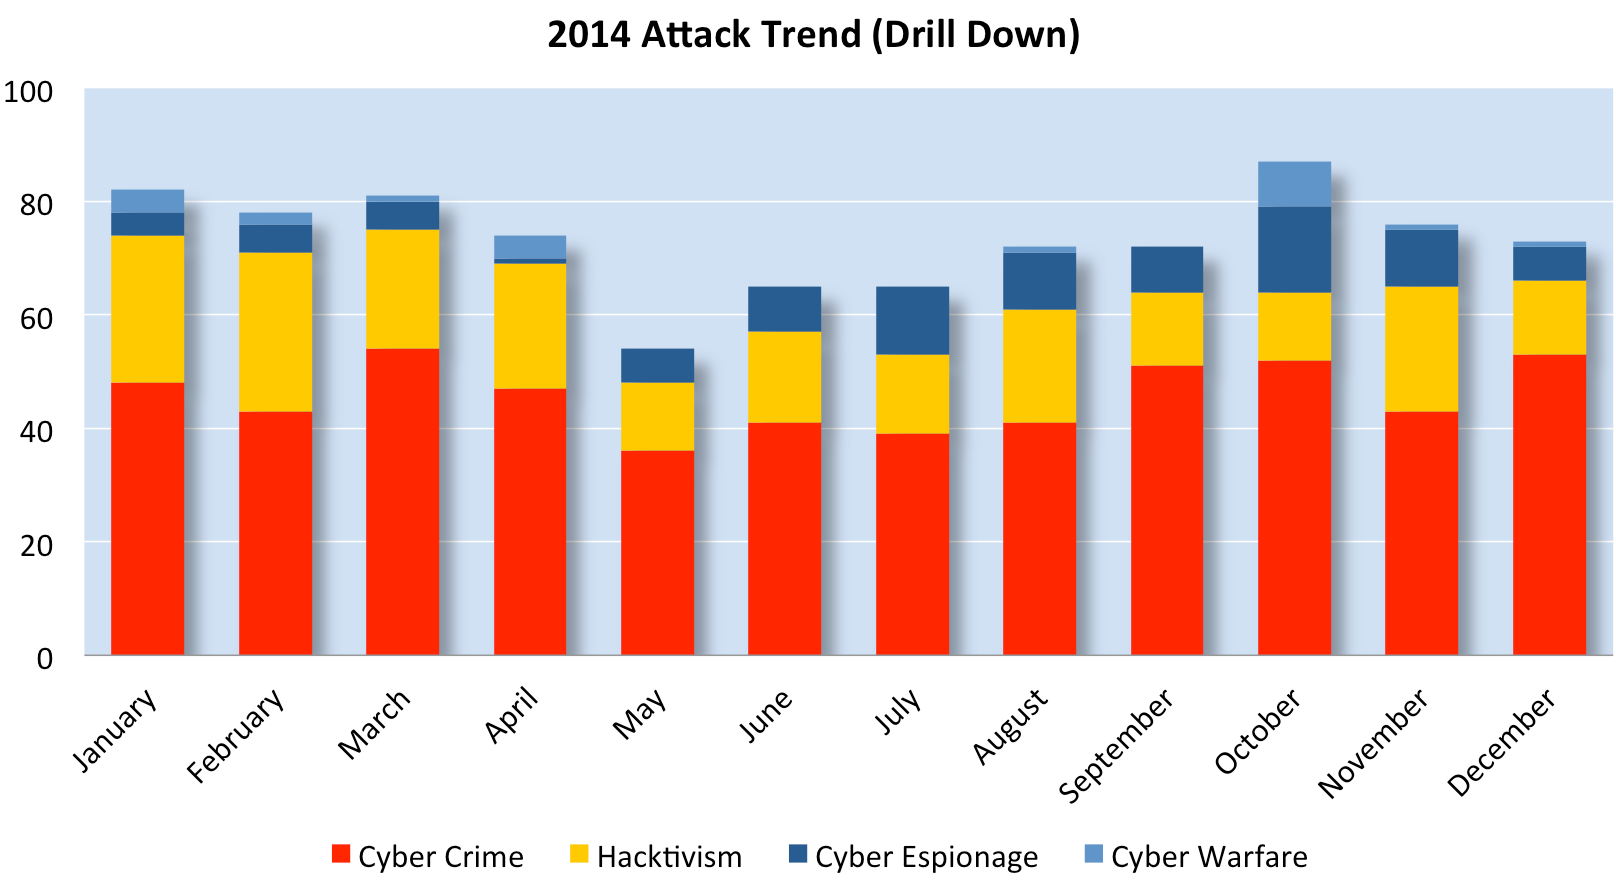
\includegraphics[scale=0.2]{Imagens/hackmageddon_trends.png}
		\caption{Difusão}
	\end{minipage}
	\begin{minipage}{.5\textwidth}
		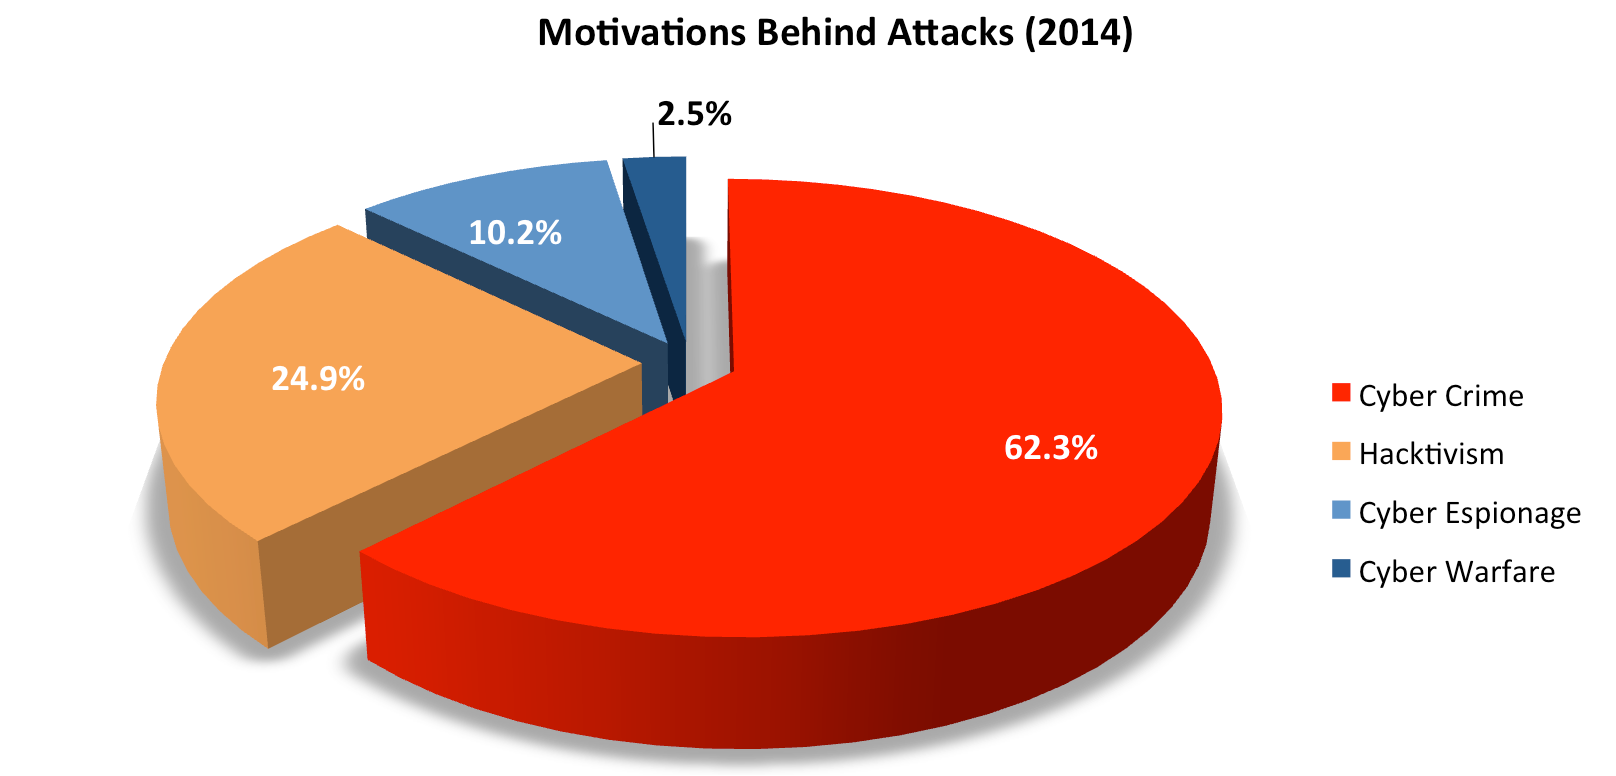
\includegraphics[scale=0.2]{Imagens/hackmageddon_motivation.png}
		\caption{Motivação}
	\end{minipage}
	\begin{minipage}{.5\textwidth}
		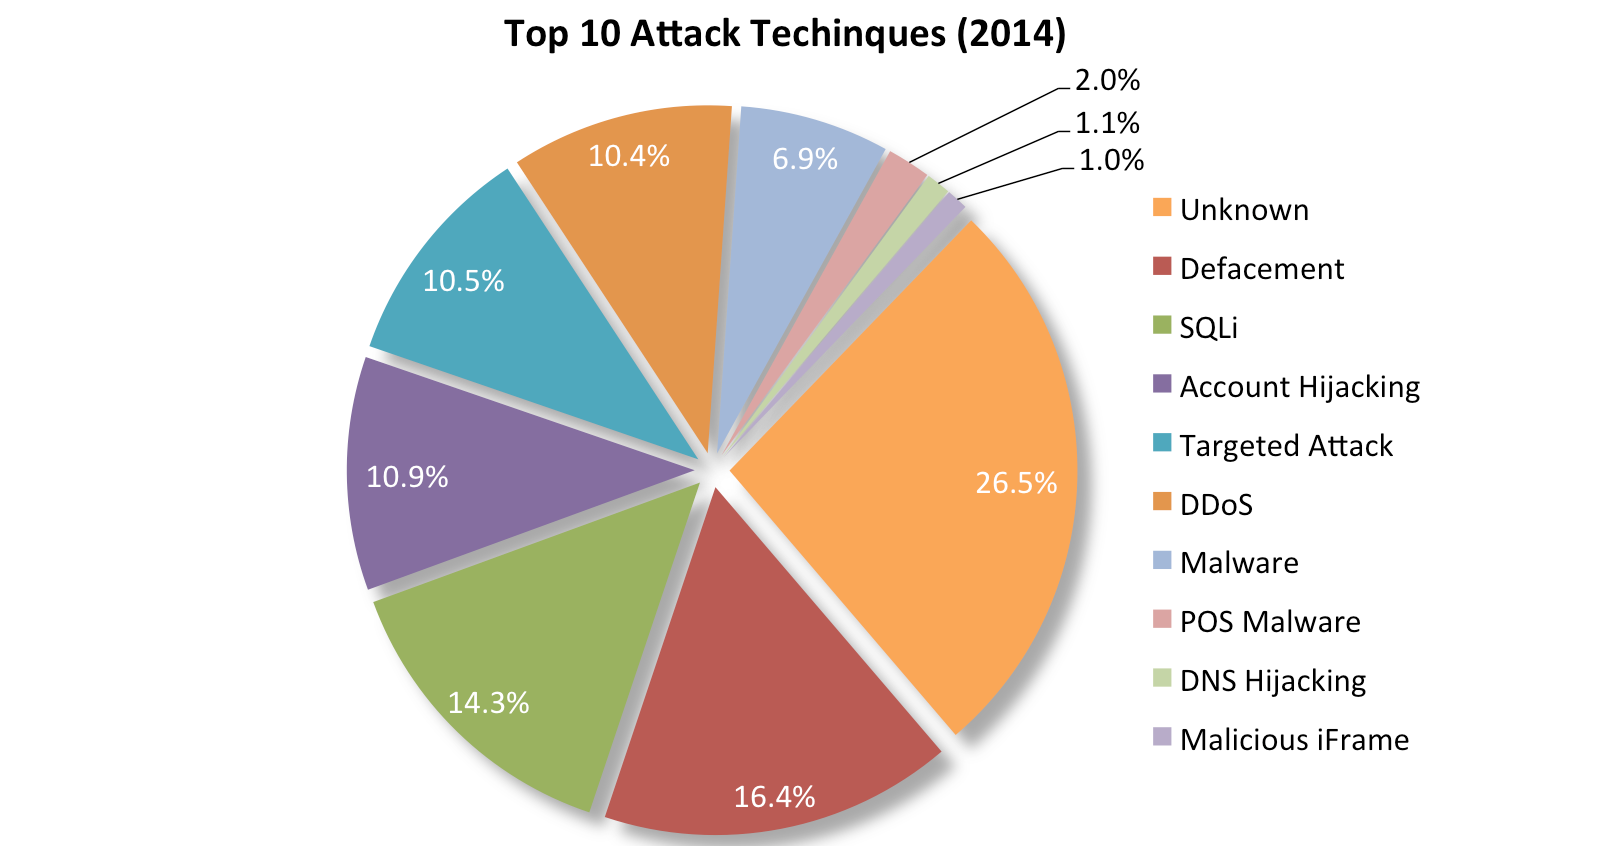
\includegraphics[scale=0.2]{Imagens/hackmageddon_techniques.png}
		\caption{Técnicas}
	\end{minipage}
	\begin{minipage}{.5\textwidth}
		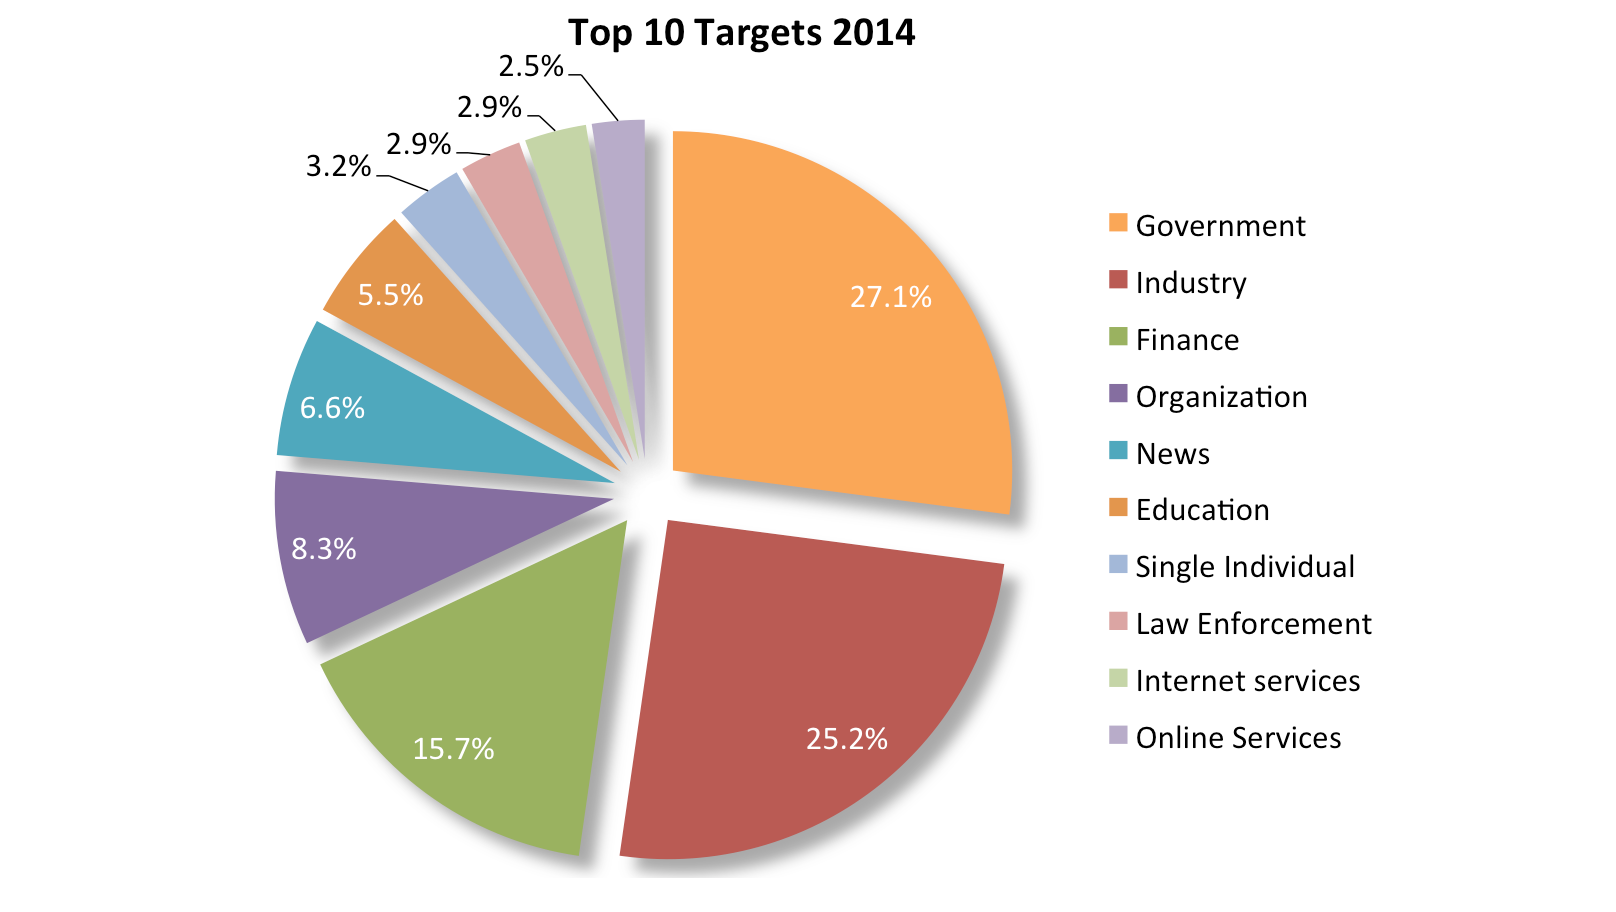
\includegraphics[scale=0.2]{Imagens/hackmageddon_targets.png}
		\caption{Alvos}
	\end{minipage}
\end{figure}

\begin{description} 
	\item[Figura 1] . 
	\item[Figura 2] .
	\item[Figura 3] .
	\item[Figura 4] The third etc 
	\ldots 
\end{description}

Os riscos são avaliados de acordo com as chances de um quebra de segurança  ocorrer e com os custos envolvidos para tratá-lo. Técnicas de defesa vêm sendo aprimoradas, porém ainda existem diversas limitações que as impedem de estarem efetivamente preparadas para o qualquer tipo de ataque \cite{CeC}, sendo assim necessário  soluções inovadoras para tratar os níveis de ameaças atuais e futuras. 

A necessidade de se proteger contra estes riscos de ataques acabou despertando interesse por ferramentas automatizadas para se detectá-los e preveni-los.

Este cenário é a principal motivação deste trabalho que consiste em propor, implementar e mensurar resultados de uma solução para treinamento de RNA para detecção e prevenção de intrusão.





\section{Escopo}

As ferramentas de detecção de intrusão são chamadas de IDS (Intrusion Detection System), seu trabalho é monitorar as atividades e analisar os eventos em uma rede em busca de anomalias que sugiram uma invasão. Estes não costumam executar qualquer ação para impedir intrusões, sua principal função é alertar os administradores de sistemas que há uma possível violação de segurança, sendo desta forma uma ferramenta passiva.
Existem as ferramentas de prevenção de intrusão, que são conhecidas como IPS (Intrusion Prevention System) estas são ferramentas que assim como IDS analisam o trafego e os eventos de uma rede, porem reagem de forma a bloquear o acesso ou atividade maliciosa, senso assim uma ferramenta ativa.

Podemos classificar os IDS da seguinte forma.

Baseado em Host ou rede, onde o primeiro faz uso de arquivos de log para cada computador individualmente e o segundo captura pacotes que trafegam na rede para analisar seu conteúdo.

Online ou Offline, onde um é capaz de detectar e marcar um intruso enquanto a esta sendo realizada a intrusão, e o outro analisa registros após o evento ocorrer e indica que houve uma violação de segurança tinha ocorrido desde a última verificação, respectivamente.

Baseado em abuso ou anomalia, onde por anomalia o sistema identifica comportamento fora do padrão, e por abuso compara as atividades na rede com comportamentos de ataques já conhecidos.

A maioria dos métodos utilizados para detecção são baseados em inteligencia artificial (AI), entre as varias técnicas conhecidas de AI, a que tem tido melhores resultados e consequentemente mais usada é a de Redes Neurais Artificiais (RNA)\cite{Jake-Ryan}\cite{Stampar}.

As RNA são uma classe de algorítimos para aprendizado de maquina (AM), usada para realizar classificação de dados. A rede neural é treinada de forma a dar mais importância para as principais características de uma determinada instancia de um problema, para ajudar a classificar os dados que ainda estão por vir. 
RNAs tem sido utilizadas com sucesso na detecção de intrusão \cite{Zhang} \cite{Tong} \cite{Wonil}, porem elas necessitam de uma quantidade substancial de dados para realizar o treinamento, a partir desse treinamento que ela passara a ter capacidade de identificar os padrões para posteriormente receber os dados novos para classificação.




\section{Justificativa}

Muitas técnicas de AI tem sido utilizadas para IDS/IPS, a mais utilizada e a RNA\cite{Stampar}, porem existem tipos de ataques que não são facilmente detectados, por ocorrerem com menor frequência, tendo poucas entradas para o treino da RNA\cite{CeC}, resultando em mais erros,  por esse motivo escolhemos trabalhar de forma a aprimorar seus resultados. 


\section{Objetivos}

O objetivo deste trabalho é propor uma forma de aprimorar o sistema de aprendizado de redes neurais artificiais para detecção e prevenção de intrusão. 
Para isso sera necessário, gerar uma base em um ambiente controlado para testes específicos, implementar uma solução de IPS/IDS que utilize RNA, implementar uma metodologia de treinamento, realizar o treino da RNA e por fim comparar resultados com outras técnicas de treinamento para RNA.


\section{Método de trabalho}

Utilizaremos a base de dados de trafego em rede KDD Cup 99\cite{KDDCup99}, por ser uma das bases mais completas e amplamente utilizada nos testes de IDS, sera essencial para se realizar uma comparação consistente de resultados.

Para gerar nossa base mais especifica iremos monitorar um ambiente de rede durante um período de tempo, no qual serão realizados alguns ataques controlados periodicamente, deste sera gerado um log que usaremos no nosso sistema.

Desenvolver uma solução para analise dos pacotes e eventos de uma rede, esta sera desenvolvida em Go, utilizara RNA para classificar as atividades na rede.

Realizar treinamento em ambas as bases de dados, serão formas diversificadas de treinamento, sera feito uma comparação de acertos/erros e tempo necessário para treino.

Faremos uma comparação de desempenho e efetividade de nossa solução e algumas que temos hoje.

\section{Organização do trabalho}

Este trabalho esta dividido em trés partes.
Na próxima seção, sera apresentado o estado da arte, onde sera revisado a literatura sobre detecção e prevenção de intrusão utilizando RNA.

Logo apos teremos a proposta  de forma mais detalhada do que é pretendido realizar na próxima etapa do trabalho.

Por fim um cronograma de controle sobre como prosseguira a segunda etapa deste trabalho.

